% =====================================================================
% 2.6 PROTOCOLO EXPERIMENTAL e 2.7 RESULTADOS E DISCUSSÃO
% Números extraídos de:
%   dados/processados/relatorio_experimento_sintetico_2026.md (perfil v1)
%   dados/processados/relatorio_experimento_sintetico_2026_v2_hp.md (perfil v2)
%   dados/processados/piloto_optframe_20260904_final/ (piloto nativo, v1)
%   dados/processados/piloto_optframe_20260907_204501/ (piloto nativo, v2)
%   dados/processados/diagnostico_curricular_2026/ e h8_trajetorias_2026/
% =====================================================================
\subsection{Protocolo experimental}
\label{subsec:protocolo}

Os experimentos realizados até o momento usam os perfis sintéticos v1 e v2 descritos na Seção~\ref{subsubsec:perfis}. Em cada perfil, a grade observada de 2026 é avaliada com as mesmas \textit{proxies} das soluções geradas e serve de referência, chamada aqui de \textit{baseline}. A melhoria gulosa é executada uma vez, e sua saída é a solução inicial de todas as buscas.

SA, ILS e VNS de referência foram executados com cinco sementes (101, 202, 303, 404 e 505) e orçamento de 1.500 avaliações por execução. O SA usou $T_0=10^6$ e $\alpha=0{,}997$. O ILS usou perturbação de três movimentos e busca local de 30 tentativas, e o VNS usou a mesma busca local. No piloto do SA nativo, cada busca teve dez segundos e partiu da mesma solução gulosa, com os parâmetros da seção anterior. As métricas registradas são o total de violações fortes e sua decomposição, o déficit de H12, cada critério fraco, o tempo de execução e o número de avaliações.

As execuções usaram Python 3.14.7 e OptFrame 5.1.0. \pendente{informar processador, memória e sistema operacional da máquina usada.} Os tempos servem apenas como ordem de grandeza, pois as implementações e os critérios de parada diferem entre as buscas de referência e a nativa.

\pendente{definir o protocolo final na instância definitiva: número de execuções por configuração, orçamento comparável entre implementações (avaliações ou tempo), calibração de parâmetros e teste estatístico usado na comparação.}

Também está planejado um estudo da ordem de planejamento das grades, em três cenários. No cenário E1, a grade de CC é otimizada e congelada antes da otimização das decisões ainda livres de SI. O cenário E2 usa a ordem inversa, e o cenário E3 otimiza as duas grades simultaneamente. A comparação entre E1 e E2 mede o custo de planejar uma grade depois da outra, que tende a crescer com o número de turmas compartilhadas. \pendente{executar E1--E3 ou retirá-los do escopo e dos objetivos específicos.}

\subsection{Resultados e discussão}
\label{subsec:resultados}

Os resultados desta seção são preliminares. Eles foram obtidos sobre perfis sintéticos e servem para validar o método, e não para recomendar uma grade à instituição. \pendente{substituir ou complementar esta seção com os resultados da instância definitiva.}

\subsubsection{Perfil v1: horários de obrigatórias fixos}

A Tabela~\ref{tab:resultado_v1} compara o \textit{baseline}, a melhoria gulosa e a melhor execução de cada meta-heurística no perfil v1. A grade observada, avaliada com as \textit{proxies}, apresenta 27 violações fortes: três conflitos de sala, dez conflitos curriculares e 14 docentes do universo sintético abaixo do mínimo anual. A melhoria gulosa reduziu esse total para 12, uma redução de 55,6\%, e também diminuiu dias com aula, janelas e desperdício de capacidade.

\begin{table}[htbp]
  \centering
  \caption{Perfil v1: \textit{baseline}, melhoria gulosa e melhor execução de cada meta-heurística. Fonte: elaborada pelo autor (2026).}
  \label{tab:resultado_v1}
  \small
  \setlength{\tabcolsep}{4pt}
  \begin{tabular}{lrrrrrrrrrr}
    \toprule
    \textbf{Configuração} & \textbf{Hard} & \textbf{Sala} & \textbf{Prof.} & \textbf{Curr.} & \textbf{H12} & \textbf{Dias} & \textbf{Jan.} & \textbf{Desp.} & \textbf{Rod.} & \textbf{Pref.} \\
    \midrule
    \textit{Baseline} & 27 & 3 & 0 & 10 & 14 & 233 & 46 & 3.521 & 38 & 79,28 \\
    Guloso            & 12 & 0 & 0 & 10 &  2 & 215 & 36 & 2.548 & 33 & 76,05 \\
    SA                & 10 & 0 & 0 & 10 &  0 & 230 & 80 & 3.453 & 29 & 68,53 \\
    ILS               & 11 & 0 & 0 & 10 &  1 & 217 & 31 & 2.548 & 32 & 76,05 \\
    VNS               & 11 & 0 & 0 & 10 &  1 & 214 & 29 & 2.544 & 32 & 74,38 \\
    \bottomrule
  \end{tabular}

  \vspace{0.2cm}
  \parbox{0.95\textwidth}{\footnotesize Legenda: Hard = total de violações fortes; Sala, Prof. e Curr. = conflitos de sala, de professor e curriculares; H12 = docentes abaixo do mínimo anual; Dias = combinações professor--semestre--dia com aula; Jan. = janelas; Desp. = desperdício estimado de capacidade; Rod. = repetições professor--disciplina nos dois semestres; Pref. = preferência atendida, ponderada pela prioridade (maior é melhor). Capacidade, recursos e descanso não tiveram violações.}
\end{table}

O SA obteve o menor número de violações fortes. Sua melhor execução, com a semente 303, chegou a 10 violações, uma redução de 62,96\% em relação ao \textit{baseline}, e eliminou os déficits de H12. As dez violações restantes são exatamente os conflitos curriculares do \textit{baseline}. Elas não podem ser corrigidas neste perfil, porque as turmas envolvidas são obrigatórias e têm horário fixo. Para zerar H12, porém, o SA aceitou mais janelas (de 36 na solução gulosa para 80) e reduziu a preferência atendida. ILS e VNS deixaram um docente abaixo do mínimo, mas preservaram melhor os critérios fracos, com menos janelas que o próprio \textit{baseline}.

\subsubsection{Perfil v2: horários de obrigatórias flexíveis}

A Tabela~\ref{tab:resultado_v2} apresenta a mesma comparação no perfil exploratório v2. Com os horários das obrigatórias flexíveis dentro dos dias do setor, a melhoria gulosa reduziu as violações fortes de 27 para 4, uma redução de 85,2\%. A melhor execução do SA, com a semente 505, não apresentou nenhuma violação forte contabilizada: eliminou os conflitos de sala e curriculares e atendeu a carga mínima de todo o universo sintético de H12.

\begin{table}[htbp]
  \centering
  \caption{Perfil v2 (exploratório): \textit{baseline}, melhoria gulosa e melhor execução de cada meta-heurística. Fonte: elaborada pelo autor (2026).}
  \label{tab:resultado_v2}
  \small
  \setlength{\tabcolsep}{4pt}
  \begin{tabular}{lrrrrrrrrrr}
    \toprule
    \textbf{Configuração} & \textbf{Hard} & \textbf{Sala} & \textbf{Prof.} & \textbf{Curr.} & \textbf{H12} & \textbf{Dias} & \textbf{Jan.} & \textbf{Desp.} & \textbf{Rod.} & \textbf{Pref.} \\
    \midrule
    \textit{Baseline} & 27 & 3 & 0 & 10 & 14 & 233 &  46 & 3.521 & 38 & 79,28 \\
    Guloso            &  4 & 0 & 1 &  1 &  2 & 214 &  38 & 2.540 & 32 & 76,55 \\
    SA                &  0 & 0 & 0 &  0 &  0 & 243 & 123 & 5.116 & 25 & 60,60 \\
    ILS               &  2 & 0 & 0 &  1 &  1 & 218 &  38 & 2.582 & 32 & 76,55 \\
    VNS               &  2 & 0 & 0 &  1 &  1 & 216 &  36 & 2.540 & 31 & 75,55 \\
    \bottomrule
  \end{tabular}

  \vspace{0.2cm}
  \parbox{0.95\textwidth}{\footnotesize Legenda: a mesma da Tabela~\ref{tab:resultado_v1}.}
\end{table}

Esse resultado tem custo nos critérios fracos. Em relação ao \textit{baseline}, a solução do SA aumentou as janelas de 46 para 123, o desperdício estimado de capacidade de 3.521 para 5.116 e os dias com aula de 233 para 243. A preferência atendida caiu de 79,28 para 60,60, enquanto o rodízio melhorou, com as repetições caindo de 38 para 25. A solução alterou 89 atribuições de professor, 61 padrões de horário e 196 salas de encontros em relação à grade observada. ILS e VNS terminaram com duas violações, mas mantiveram janelas e desperdício próximos aos da solução gulosa.

A Figura~\ref{fig:hard} resume as violações fortes nos dois perfis. A comparação mostra que a liberdade para mover os horários das obrigatórias é o que permite eliminar os conflitos curriculares. As hipóteses que a sustentam, porém, ainda dependem de validação do orientador.

\begin{figure}[htbp]
  \centering
  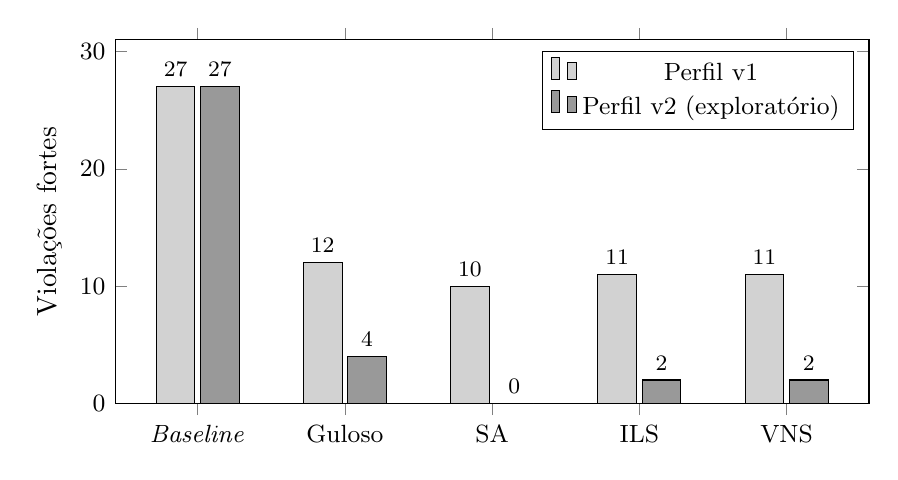
\begin{tikzpicture}
    \begin{axis}[
        ybar,
        bar width=14pt,
        width=0.92\textwidth,
        height=6.2cm,
        ymin=0, ymax=31,
        ylabel={Violações fortes},
        symbolic x coords={Baseline,Guloso,SA,ILS,VNS},
        xticklabels={\textit{Baseline},Guloso,SA,ILS,VNS},
        xtick=data,
        enlarge x limits=0.14,
        nodes near coords,
        every node near coord/.append style={font=\footnotesize},
        legend style={at={(0.98,0.97)}, anchor=north east, font=\small},
        tick label style={font=\small},
      ]
      \addplot[fill=gray!35, draw=black] coordinates {(Baseline,27) (Guloso,12) (SA,10) (ILS,11) (VNS,11)};
      \addplot[fill=gray!80, draw=black] coordinates {(Baseline,27) (Guloso,4) (SA,0) (ILS,2) (VNS,2)};
      \legend{Perfil v1, Perfil v2 (exploratório)}
    \end{axis}
  \end{tikzpicture}
  \caption{Violações fortes do \textit{baseline}, da melhoria gulosa e da melhor execução de cada meta-heurística nos perfis sintéticos. Fonte: elaborada pelo autor (2026).}
  \label{fig:hard}
\end{figure}

\subsubsection{Variação entre sementes}

A Tabela~\ref{tab:sementes} resume as cinco execuções de cada método. Nos dois perfis, o SA teve a menor média de violações fortes e foi o único método a atender H12 em alguma execução. No perfil v1, isso ocorreu em três das cinco sementes; no perfil v2, em quatro. ILS e VNS terminaram com pelo menos um docente abaixo do mínimo em todas as execuções. Os resultados por semente estão no Apêndice~C.

\begin{table}[htbp]
  \centering
  \caption{Resumo das cinco execuções por método: média e desvio-padrão amostral das violações fortes, melhor resultado, execuções que atenderam H12, déficit médio de H12 e tempo médio. Fonte: elaborada pelo autor (2026).}
  \label{tab:sementes}
  \small
  \begin{tabular}{llrrrrr}
    \toprule
    & & \multicolumn{2}{c}{\textbf{Violações fortes}} & \textbf{H12} & \textbf{Déficit} & \textbf{Tempo} \\
    \cmidrule(lr){3-4}
    \textbf{Perfil} & \textbf{Método} & \textbf{média $\pm$ dp} & \textbf{melhor} & \textbf{atendida} & \textbf{médio} & \textbf{(s)} \\
    \midrule
    v1 & SA  & 10,4 $\pm$ 0,55 & 10 & 3/5 & 0,4 & 5,8 \\
    v1 & ILS & 11,2 $\pm$ 0,45 & 11 & 0/5 & 1,4 & 8,3 \\
    v1 & VNS & 11,2 $\pm$ 0,45 & 11 & 0/5 & 1,2 & 8,7 \\
    \midrule
    v2 & SA  & 1,0 $\pm$ 0,71 & 0 & 4/5 & 0,2 & 5,2 \\
    v2 & ILS & 2,6 $\pm$ 0,55 & 2 & 0/5 & 1,4 & 5,4 \\
    v2 & VNS & 2,8 $\pm$ 0,84 & 2 & 0/5 & 1,0 & 5,6 \\
    \bottomrule
  \end{tabular}
\end{table}

Com apenas cinco sementes e parâmetros não calibrados, essas diferenças não permitem afirmar superioridade estatística de um método. Ainda assim, o padrão é consistente nos dois perfis. O SA, que aceita pioras nos critérios fracos, alcança a viabilidade com mais frequência. ILS e VNS, que só aceitam melhoras, preservam melhor a qualidade da solução gulosa. \pendente{aplicar teste estatístico com mais execuções na instância definitiva.}

\subsubsection{Piloto com o SA nativo do pyoptframe}

A Tabela~\ref{tab:piloto} compara o SA de referência e o SA nativo, ambos partindo da mesma solução gulosa. Todas as soluções nativas passaram pela validação estrutural e pela conferência entre os dois avaliadores. A reexecução do SA de referência no piloto reproduziu, semente a semente, os mesmos resultados do experimento anterior, o que confirma o determinismo da implementação em Python sob semente fixa.

\begin{table}[htbp]
  \centering
  \caption{Piloto do SA nativo do pyoptframe: violações fortes por semente, na ordem 101, 202, 303, 404 e 505. Fonte: elaborada pelo autor (2026).}
  \label{tab:piloto}
  \small
  \begin{tabular}{llcrr}
    \toprule
    \textbf{Perfil} & \textbf{Implementação} & \textbf{Violações por semente} & \textbf{Melhor} & \textbf{Avaliações} \\
    \midrule
    v1 (guloso: 12) & SA de referência & 11, 10, 10, 10, 11 & 10 & 1.500 \\
                    & SA nativo        & 12, 12, 10, 12, 11 & 10 & 422 a 471 \\
    \midrule
    v2 (guloso: 4)  & SA de referência & 2, 1, 1, 1, 0 & 0 & 1.500 \\
                    & SA nativo        & 2, 3, 4, 3, 4 & 2 & 341 a 369 \\
    \bottomrule
  \end{tabular}
\end{table}

No perfil v1, o SA nativo alcançou o mesmo melhor resultado da referência em uma das cinco sementes, mas três execuções terminaram sem melhorar a solução gulosa. No perfil v2, que tem um espaço de busca maior, ele ficou atrás da referência em todas as sementes, e duas execuções também não melhoraram a solução gulosa. Os dois arranjos, porém, não são diretamente comparáveis. O SA nativo teve dez segundos por execução e realizou de 341 a 471 avaliações, enquanto a referência usou 1.500 avaliações em cerca de cinco a seis segundos. Os esquemas de resfriamento e as temperaturas também diferem. Uma hipótese para a menor vazão do motor nativo é o custo da ponte entre Python e o núcleo do OptFrame, que ainda precisa ser medido. O piloto, portanto, valida a integração, mas não estabelece qual implementação é melhor.

\subsubsection{Conflitos curriculares e a interpretação de H8}
\label{subsubsec:h8}

Os dez conflitos curriculares da grade observada foram diagnosticados individualmente. Eles ocorrem em dois grupos da grade de SI: quatro sobreposições no primeiro período em cada semestre e duas no sexto período em 2026/1. Os horários envolvidos coincidem nas extrações dos PDFs e na coleta das páginas públicas, portanto as sobreposições são reais. Em todos os casos, porém, há uma escolha de uma seção por disciplina sem choque. Em 2026/1, por exemplo, a turma TCC00332-A1 coincide com TCC00354-A1, mas a combinação de TCC00332-A1 com TCC00354-B1 evita o choque.

Isso expõe uma questão de modelagem. O contador atual de H8 exige que nenhuma oferta de disciplinas diferentes do grupo se sobreponha, mesmo quando essas ofertas são seções alternativas. Uma interpretação alternativa exigiria apenas que o aluno tivesse ao menos uma trajetória viável, isto é, uma escolha de seções sem choque. Essa segunda leitura é mais próxima da matrícula real, mas exige modelar a elegibilidade das seções e, para garantir atendimento coletivo, a demanda e as vagas.

Para apoiar essa decisão, foi implementada uma verificação paralela de H8 por trajetória, que não altera o avaliador usado na busca. Para cada grupo curricular, ela procura uma seção utilizável de cada disciplina obrigatória do período, sem choques entre as escolhidas. Como filtro provisório de elegibilidade, considera-se utilizável a seção com vagas ofertadas para o curso do grupo. A Tabela~\ref{tab:trajetorias} mostra o resultado para os 32 grupos da grade observada, que correspondem a oito períodos de cada curso nos dois semestres.

\begin{table}[htbp]
  \centering
  \caption{Verificação de H8 por trajetória nos 32 grupos curriculares de 2026. Fonte: elaborada pelo autor (2026).}
  \label{tab:trajetorias}
  \small
  \begin{tabular}{p{6cm}rrr}
    \toprule
    & \multicolumn{3}{c}{\textbf{Grupos curriculares}} \\
    \cmidrule(lr){2-4}
    \textbf{Dados considerados} & \textbf{com trajetória} & \textbf{sem trajetória} & \textbf{incompletos} \\
    \midrule
    Somente o recorte CC/SI & 7 & 0 & 25 \\
    Recorte com complemento da coleta web & 22 & 0 & 10 \\
    \bottomrule
  \end{tabular}
\end{table}

No recorte, a maioria dos grupos fica inconclusiva porque as disciplinas de outros departamentos não estão na instância. Com o complemento da coleta web, que só acrescenta disciplinas ausentes e nunca altera horários da solução, 22 grupos têm trajetória e nenhum grupo fica comprovadamente sem trajetória. Os dez grupos restantes têm, cada um, uma disciplina sem turma utilizável nos dados. Esse diagnóstico não comprova vagas suficientes nem atendimento de todos os alunos, mas indica que, nos grupos afetados, os conflitos contados por H8 na grade observada não impedem que um aluno curse o período. \pendente{registrar a decisão do orientador sobre a semântica de H8 e, se for o caso, incorporar a verificação por trajetória ao avaliador.}

\subsubsection{Discussão}

Três observações emergem dos resultados preliminares. A primeira é que a melhoria gulosa responde pela maior parte do ganho: nos dois perfis, ela removeu mais da metade das violações fortes com uma única passagem. A segunda é que os métodos se complementam. O SA é mais eficaz em alcançar viabilidade, enquanto ILS e VNS preservam melhor os critérios fracos, o que sugere um fluxo combinado em que o SA busca a viabilidade e ILS ou VNS refinam a solução.

A terceira observação é que existe um conflito claro entre viabilidade e conforto docente. Como a chave lexicográfica prioriza qualquer redução de violações fortes, soluções viáveis podem ter mais janelas, mais dias de aula e menos preferências atendidas. Esse comportamento é coerente com a formulação, mas reforça a necessidade de definir com o orientador quais regras são de fato inegociáveis e quais pesos devem equilibrar os critérios fracos.

Os resultados têm limitações importantes. Capacidades, recursos, habilitações, prioridades e o universo de H12 são \textit{proxies}, e as capacidades são apenas limites inferiores. O perfil v2 depende de hipóteses ainda não validadas. A instância contém apenas uma turma de outro departamento, de modo que H8 ainda não considera a maior parte das disciplinas externas das grades. Por fim, o número de execuções é pequeno e os orçamentos das implementações de referência e nativa não são equivalentes. \pendente{revisar esta discussão após os experimentos definitivos, incluindo gráficos de convergência e a comparação com a grade observada na instância oficial.}
